% Look!  A mock introduction

% The introduction is one of the most important pieces of your thesis.  Here is a place for you to introduce the problem(s) on which you have worked and place them in the larger context of your field.  You should aim to ensure that this section is completely understandable to virtually anyone - and certainly anyone with a sophomore-level grasp of physics.  Presumably this will include references to the literature.

% In addition to setting your work into context, a second good idea for your introduction is to give a short outline for what the rest of your thesis will discuss.  This is often done in the closing paragraph(s) of the introduction with sentences like ``In the following chapters \ldots " and ``Chapter 2 discusses \ldots"  Tremendous detail is not required in this outline, but rather just a brief road map for the rest of the document.

This thesis centers on the modeling of Passive Daytime Radiative Cooling Devices (PDRCs) utilizing the COMSOL Multiphysics™ software. While all objects with a temperature above absolute zero emit blackbody radiation, PDRCs are distinct in their ability to efficiently radiate heat in the mid-infrared range where the Earth's atmosphere is most transparent. This allows PDRCs to effectively transfer heat directly to the cold sink of outer space during daylight hours, without the need for electrical energy. Therefore, PDRCs hold the promise of addressing two significant challenges: the energy crisis and global warming. % rephrased

\section{Cooling is Critical}
Over the years, cooling has become more critical to humans due to global warming, rapid population growth and industrial development \cite{chen_passive_2022}. Various methods exist for cooling buildings, ranging from traditional practices, such as shading and solar orientation, to the use of electric fans. The most advanced approach is air conditioning (AC), encompassing systems that enhance indoor thermal comfort and air quality. While mechanical cooling techniques date back to the 19th century, widespread adoption of air conditioning began in the 1950s, driven by improved performance, affordability, and economic prosperity, primarily in the United States \cite{international_energy_agency_future_2018}.

Modern AC systems vary widely in size and cost, catering to individual rooms or entire buildings, with electricity being the predominant power source. Today, the largest concentration of cooling systems is found in urban areas, both in industrialized nations and emerging economies, reflecting the higher population density and greater demand for climate control in these regions \cite{international_energy_agency_future_2018}. 

Particularly in the realm of residential air conditioners (ACs), China emerges as the foremost market with a staggering sale of 41 million units. Following China, Japan and the European Union represent the subsequent largest markets for residential ACs. However, there is a significant uptick in sales within various emerging economies, notably in Asia (see figure \ref{fig:sales_acs}).

Global sales of ACs have exhibited consistent growth in recent years. Over the period from 1990 to 2016, annual AC sales experienced a nearly fourfold increase, reaching 135 million units. In 2016, China emerged as the leading market in terms of AC capacity sales, totaling nearly 390 gigawatts (53 million units) \cite{international_energy_agency_future_2018}. % rephrased

\begin{figure}
  \centering
  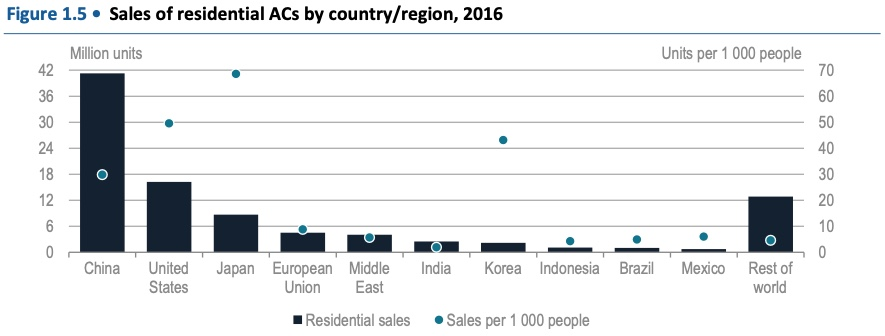
\includegraphics[width=0.8\textwidth]{Chapters/Figures/Sales of Residential ACs by Country or Region, 2016.jpg}
  \caption[Sales of Residential ACs by Country or Region, 2016]{Sales of Residential ACs by Country or Region, 2016. Source: \cite{international_energy_agency_future_2018}.}
  \label{fig:sales_acs}
\end{figure}

The growing demand for cooling is significantly influencing power systems, primarily due to the reliance on electricity-driven fans or air conditioners to meet cooling requirements. The escalating demand for air conditioning, in particular, not only elevates overall electricity consumption but also contributes to higher peak electricity loads. Additionally, the emission of greenhouse gases (GHGs) from ACs occurs through refrigerant leakage or improper disposal. It's noteworthy that these refrigerants are potent GHGs with adverse implications for climate change \cite{international_energy_agency_future_2018}. % (INTERNATIONAL ENERGY AGENCY, 2018) % rephrased

Improving the efficiency of air conditioning systems (ACs) is pivotal in mitigating peak electricity demand, thereby resulting in decreased emissions and associated financial implications. Endeavors focused on enhancing cooling efficiency necessitate a thorough assessment of the comparative costs linked to diverse cooling technologies. % rephrased

\section{Radiative Cooling}

\begin{figure}
  \centering
  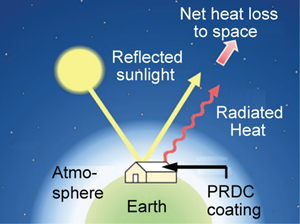
\includegraphics[width=0.4\textwidth]{Chapters/Figures/Schematic for Radiative Cooling.png}
  \caption[Schematic for Radiative Cooling] {Schematic for Radiative Cooling. Source: \cite{yang_passive_2020}}
  \label{fig:PDRC_Schematic}
\end{figure}

Objects with temperatures above absolute zero emit blackbody radiation, with a spectrum that depends on their temperature as governed by Planck's law. While the emitted radiation covers a range of wavelengths, it is not uniformly distributed across all wavelengths. Radiative passive cooling occurs when objects emit more radiation, particularly in the infrared spectrum, than the combined radiation they absorb, which includes both blackbody and solar radiation. Thus radiative passive cooling is an electricity-free method for cooling terrestrial entities \cite{yang_passive_2020}.

The heat emitted by these objects, which exceeds the heat they absorb, is transferred to outer space via thermal radiation, leveraging the substantial temperature difference between Earth (approximately 300 K) and outer space (approximately 3 K) (See figure \ref{fig:PDRC_Schematic} for net heat loss to space). This process efficiently exchanges heat with the infinite cold reservoir of deep space, achieving cooling without any energy consumption \cite{chen_passive_2022}.

Passive radiative cooling can be realized even during the daytime, necessitating precise tuning of optical properties across a broad spectrum of wavelengths, from ultraviolet to mid-infrared (see figure \ref{fig:ideal_PDRC_properties}). As a result, achieving effective passive daytime radiative cooling imposes stringent requirements on materials and structures to mitigate solar heating \cite{yang_passive_2020}:

\begin{enumerate} 
\item Minimal absorptivity ($\alpha$) approaching 0\% (equivalent to nearly 100\% reflectance, $R$) in the solar spectrum, ranging from 0.3–2.5 $\mu m$. This characteristic ensures that the surface absorbs minimal solar energy during daylight, thereby reducing the heat gained by the PDRC.
\item High thermal radiation in the atmospheric transparency window, with an emittance ($\varepsilon$) close to 1 within the long-wavelength infrared (LWIR) transmission window of the atmosphere ($\lambda$ = 8–13 $\mu m$). This range is significant due to the atmosphere's partial transparency and minimal infrared absorption by gas molecules in this spectrum.
\item An emittance ($\varepsilon$) close to 0 in other mid-infrared wavelengths, such as 5–8 $\mu m$ and those greater than 13 $\mu m$. This characteristic is crucial due to the atmosphere's opacity in these spectral ranges.
\end{enumerate}

% NB: Using [ht!] tells LaTeX to try to place the figure here, but if that's not possible, then at the top of the page, and the ! overrides LaTeX's internal parameters for deciding on figure placements. This gives you the best chance of having the figure appear right after your enumerated list, although it's not a guarantee because LaTeX might still decide to move the figure based on its page layout algorithms.
\begin{figure}[ht!]
  \centering
  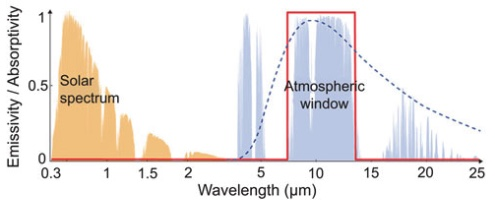
\includegraphics[width=0.4\textwidth]{Chapters/Figures/Ideal Optical Properties of a Radiative Cooling Surface.jpg}
  \caption[Ideal Optical Properties of a Radiative Cooling Surface]{Ideal Optical Properties of a Radiative Cooling Surface. Source: \cite{yang_passive_2020}}
  \label{fig:ideal_PDRC_properties}
\end{figure}


% -- SECTION 1.3: PREVIOUS PROJECT WORK AND PROJECT GOALS ---

\section{Previous Project Work and Project Goals}
Research on PDRCs has been an ongoing project in the Hudgings lab. This thesis aims to build upon the work of Paul McKinley (class of 2022) and Genevieve diBari (class of 2023).

McKinley laid the groundwork by developing a rooftop testbed and the fabrication process for PDRCs (a process I plan to replicate after completing the modeling of various PDRC iterations on COMSOL). DiBari contributed by modeling PDRCs in Python and enhancing the initial outdoor testing setup.

For my thesis, the goal is to model different PDRC structures using COMSOL, exploring materials that could enhance the optical properties of an ideal PDRC device. This includes stacking materials of varying thicknesses and refractive indices on current PDRC models in the Hudgings lab to increase reflectivity ($R$). If time permits, promising PDRC models (with high $R$ and/or emissivity in the atmospheric window) will be fabricated after the modeling phase.
